\chapter{Metodologia}

Neste capítulo é apresentado o planejamento metodológico que orientará o desenvolvimento do projeto. São descritos o processo de pesquisa, as metodologias ágeis de desenvolvimento escolhidas e os artefatos de levantamento de requisitos, incluindo as histórias de usuário e a classificação por FURPS+.

\section{Processo Metodológico}

Conforme as normas estabelecidas pela Universidade de Brasília, o Trabalho de Conclusão de Curso é estruturado em duas etapas sequenciais: TCC1 e TCC2. A primeira fase dedica-se à elaboração de uma proposta de projeto tecnicamente viável para desenvolvimento e à construção do seu referencial teórico fundamental. Por sua vez, o TCC2 concentra-se na execução e implementação prática do projeto que foi definido e delineado durante a fase do TCC1.

\subsubsection{TCC1}

A organização e o detalhamento das etapas que compõem este primeiro volume do trabalho estão apresentados abaixo.

\begin{itemize}
    \item Semana do dia 15 de março de 2026: Escolher um tema.
    \item Semana do dia 22 de março de 2026: Especificar a questão no tema.
    \item Semana do dia 29 de março de 2026: Determinar uma metodologia.
    \item Semana do dia 05 de abril de 2026: Fazer revisão sistemática da bibliografia.
    \item Semana do dia 12 de abril de 2026: Fazer revisão sistemática da bibliografia.
    \item Semana do dia 19 de abril de 2026: Levantamento de requisitos.
    \item Semana do dia 26 de abril de 2026: Levantamento de requisitos.
    \item Semana do dia 03 de maio de 2026: Definir uma solução.
    \item Semana do dia 10 de maio de 2026: Definir uma solução.
    \item Semana do dia 17 de maio de 2026: Determinar a arquitetura.
    \item Semana do dia 24 de maio de 2026: Modelar artefatos.
    \item Semana do dia 31 de maio de 2026: Modelar artefatos.
    \item Semana do dia 07 de junho de 2026: Modelar artefatos.
    \item Semana do dia 14 de junho de 2026: Prototipar.
    \item Semana do dia 21 de junho de 2026: Prototipar.
    \item Semana do dia 28 de junho de 2026: Prototipar.
    \item Semana do dia 05 de julho de 2026: Revisar o trabalho realizado.
    \item Semana do dia 12 de julho de 2026: Apresentar o trabalho.
\end{itemize}

A seguir, está representado o diagrama de fluxo de atividades BPMN do atual trabalho.

\clearpage

\begin{figure}[H]
    \centering
    \caption{Raia do TCC1 do BPMN do Processo Metodológico.}
    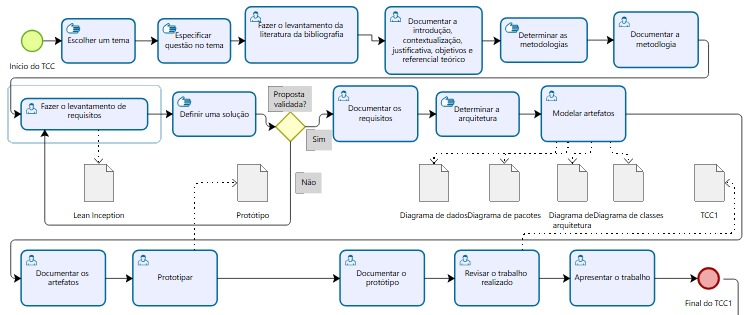
\includegraphics[width=1\textwidth]{Imagens/BPMNTCC1.png}
    \par
    Fonte: autoria própria.
    \par
    \label{(atividades-tcc1)}
\end{figure}

\subsubsection{TCC2}

A seguir, está representado o diagrama de fluxo de atividades BPMN do TCC2, que será realizado posteriormente ao atual trabalho.

\begin{figure}[H]
    \centering
    \caption{Raia do TCC2 do BPMN do Processo Metodológico.}
    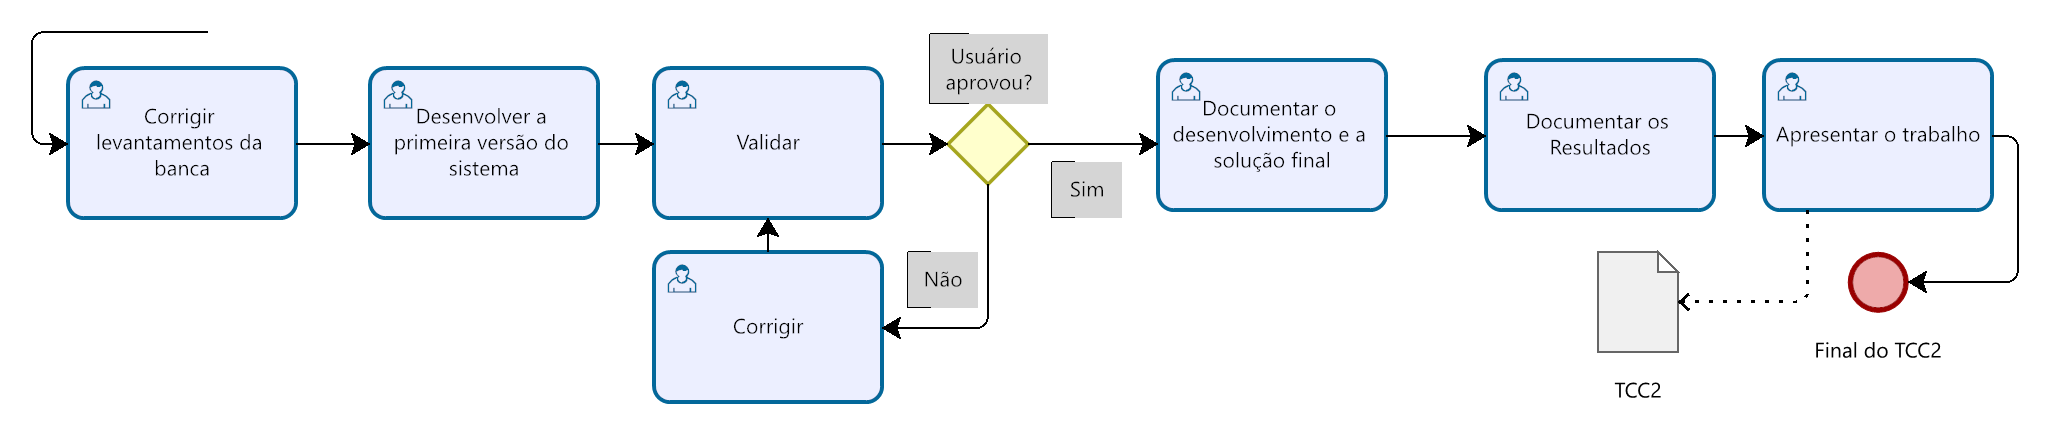
\includegraphics[width=1\textwidth]{Imagens/BPMNTCC2.png}
    \par
    Fonte: autoria própria.
    \par
    \label{(atividades-tcc2)}
\end{figure}

Portanto, podemos representar todo o fluxo de atividades de ambos os trabalhos no seguinte diagrama BPMN.

\begin{figure}[H]
    \centering
    \caption{BPMN do Processo Metodológico}
    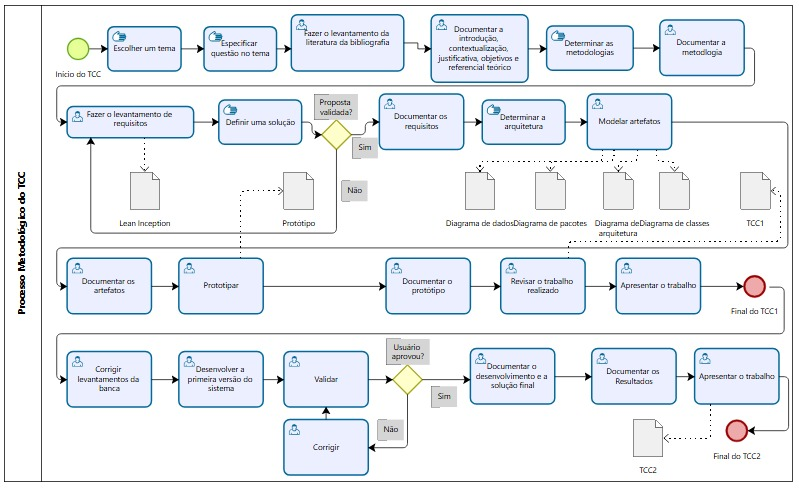
\includegraphics[width=0.9\textwidth]{Imagens/BPMNCompletoTCC.png}
    \par
    Fonte: autoria própria.
    \par
    \label{(atividades-tcc12)}
\end{figure}

\section{Metodologia de Desenvolvimento}

A escolha da metodologia de desenvolvimento de software é um pilar que define a forma como o projeto será planejado, executado e gerenciado, afetando diretamente na capacidade de entrega e na adaptação aos requisitos. Tradicionalmente, o desenvolvimento era dominado por modelos preditivos, como o modelo cascata, que exige o levantamento completo de requisitos antes da codificação em si. Contudo, o mercado de software tem migrado para abordagens mais interativas. Essa transição reflete a necessidade de lidar com a complexidade e a volatilidade do ambiente de negócios moderno, onde as necessidades dos usuários e as tecnologias evoluem rapidamente. Essa mudança para o ágil é uma tendência consolidada na educação em gerenciamento de projetos de software, acompanhando as demandas do mercado.

A metodologia ágil, representada por frameworks como Scrum, Kanban e Extreme Programming (XP), é a mais adequada para o desenvolvimento de soluções dinâmicas e centradas no usuário, como o aplicativo proposto neste trabalho. Em contraste com a rigidez do modelo cascata, o ágil valoriza a colaboração, a entrega contínua de software funcional e a adaptação a requisitos novos. Em um estudo de caso realizado em uma instituição de ensino superior, \citeonline{santos_2024} analisaram a transição do cascata para o Scrum em um curso de Gerenciamento de Projetos e demonstraram que, seguindo o Scrum, os estudantes se tornaram mais capazes de desenvolver software em equipes, com maior foco nos clientes, e adquiriram mais conhecimento em áreas fundamentais de desenvolvimento de software.

\subsection{Metodologia Ágil}

Dessa forma, a escolha por uma metodologia de desenvolvimento ágil é uma estratégia para evitar riscos e otimizar o ciclo de vida do projeto. Ao aderir a frameworks ágeis, este trabalho garante a capacidade de flexibilizar o plano de desenvolvimento, permitindo ajustes rápidos e eficientes caso surjam a necessidade de alterar ou refinar requisitos ao longo do processo. Além disso, o foco em entregas curtas e frequentes proporcionam um processo mais produtivo, onde o progresso é continuamente visível e funcional.

Contudo, o projeto proposto visa adotar as metodologias ágeis como o principal instrumento para assegurar a flexibilidade necessária e impulsionar a produtividade. Essa abordagem metodológica, conforme validada pela experiência educacional descrita por \citeonline{santos_2024}, é fundamental para desenvolver software. Focar nas necessidades do usuário e evitar os riscos de desvios de escopo ou de incompatibilidade do produto final com as demandas resultam em uma implementação mais eficiente e centrada no cliente.

\subsection{Extreme Programming (XP)}

O Extreme Programming (XP) é uma metodologia ágil, rigorosa e disciplinada, focada na entrega contínua de software em ambientes com requisitos de mudança frequente. A metodologia é definida por uma série de práticas relacionadas, agrupadas em quatro áreas centrais: Planejamento, Design, Codificação e Teste. No centro do XP está o valor da simplicidade, da comunicação constante e da motivação para refatorar o código. Essa ênfase na adaptabilidade e na qualidade do código desde o início faz do XP uma boa escolha para projetos que buscam resultados sustentáveis.

A metodologia XP é eficaz em projetos que precisam de integração intensa e rápida, como o desenvolvimento de uma plataforma que unifica várias ideias. Os processos chave do XP incluem o desenvolvimento guiado por testes e a programação em par. Essas práticas visam mitigar erros, garantir a qualidade e transferir conhecimento de forma eficiente dentro da equipe. \citeonline{sasmito_2025} demonstraram a implementação do método XP no desenvolvimento de um website para gerenciamento de pedidos de transporte de colheitas agrícolas, confirmando que o XP pode ser aplicado com sucesso para a construção de sistemas que gerenciam dados complexos e exigem alta funcionalidade.

Para o contexto deste trabalho, o XP oferece um modelo metodológico de alto desempenho, complementando o framework Scrum adaptado. O XP pode ser utilizado para definir as práticas de engenharia dentro de cada Sprint do Scrum, garantindo que a implementação dos requisitos seja feita com a máxima qualidade e menor erro técnico possível. Entretanto, devido ao escopo do projeto, não é viável adotar todas as 12 práticas do método, sendo priorizado apenas os testes TDD (\textit{Test-Driven Development}) e a refatoração.

\subsection{Test-Driven Development}

O \textit{Test-Driven Development} (TDD), ou Desenvolvimento Orientado por Testes, é uma prática essencial das metodologias ágeis que inverte a ordem tradicional de codificação. Em vez de escrever o código e depois testá-lo, o TDD exige que os desenvolvedores escrevam um teste unitário que falhe antes de escrever qualquer código. O processo segue o seguinte ciclo: o teste falha, o desenvolvedor escreve o código mínimo necessário para fazer o teste passar, e, em seguida, refatora o código para limpá-lo, mantendo a funcionalidade garantida pelos testes. Essa prática assegura que cada parte do software atenda a um requisito específico e seja verificável, promovendo uma base de código confiável.

\begin{figure}[H]
    \centering
    \caption{Ciclo de desenvolvimento TDD}
    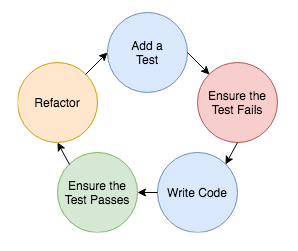
\includegraphics[width=0.6\linewidth]{Imagens/CicloTDD.png}
    \par
    Fonte: \cite{testdriven_2025}.
    \par
    \label{fig:ciclo_tdd}
\end{figure}

A principal contribuição do TDD para a qualidade do software reside em duas áreas cruciais: qualidade externa e produtividade do desenvolvedor. Ao forçar o desenvolvedor a pensar nas especificações e em cenários de uso antes de codificar, o TDD resulta em um design mais simples e modular, pois o código se torna mais fácil de testar. Essa modularidade simplifica a manutenção e a inclusão de novas funcionalidades no futuro. Embora a aplicação do TDD seja amplamente aceita no desenvolvimento de software genérico, seu uso em sistemas mais complexos, como sistemas embarcados, tem sido objeto de investigação. \citeonline{cassieri_2025}, por exemplo, investigaram os benefícios alegados do TDD, como o aumento da qualidade e da produtividade, e a forma como os desenvolvedores aplicam essa técnica em ambientes de Sistemas Embarcados.

A metodologia TDD é fundamental para o sucesso do aplicativo proposto neste trabalho, especialmente na implementação de módulos de alta complexidade, como o Algoritmo de Repetição Espaçada (SRS). A precisão dos cálculos do SRS e a correta integração do Timer Pomodoro com Gamificação não podem depender de testes manuais. O TDD garantirá que cada regra de negócio do algoritmo seja coberta por um teste, minimizando a probabilidade de erros de cálculo que poderiam comprometer todo o plano de estudo do usuário. Dessa forma, a adesão ao TDD não só eleva a qualidade do código, conforme discutido por \citeonline{cassieri_2025}, mas também fornece uma garantia metodológica de que as funcionalidades do sistema estão operando de acordo com o referencial teórico e os requisitos definidos.

\subsection{Scrum}

O Scrum é um framework ágil adaptável e muito utilizado que estabelece uma estrutura iterativa e incremental para o gerenciamento de projetos, ideal para o desenvolvimento de software. O Scrum opera através de ciclos de trabalho curtos e repetitivos chamados Sprints, geralmente com duração de duas a quatro semanas. A principal função do Scrum é facilitar a entrega rápida de valor, garantindo que o produto seja constantemente refinado com base no feedback do cliente e nos novos requisitos. O framework define papéis específicos e eventos estruturados que mantém a equipe focada e alinhada com os objetivos do projeto.

A metodologia Scrum é fundamental para este trabalho, pois o projeto exige a integração de múltiplas funcionalidades pedagógicas e tecnológicas que precisam ser desenvolvidas em fases paralelas. A aplicação do Scrum permite que cada Sprint se concentre na entrega de um incremento funcional do produto, mitigando o risco de desvios de escopo comuns em projetos de longo prazo. \citeonline{ibarra_2025} destacam em seus estudos que a aplicação do Scrum pode ser uma ferramenta eficaz para a transferência de conhecimento entre desenvolvedores, especialmente através dos eventos como o Daily Scrum e as sessões de Pair Programming.

Dessa forma, a Sprint Review será utilizada para demonstrar o incremento do software e coletar feedback do orientador, a Sprint Retrospective garantirá a melhoria contínua do processo de desenvolvimento, e, apesar do trabalho ser realizado por uma única pessoa, a documentação dos processos e impedimentos arquivam conhecimentos importantes para manter o cronograma de desenvolvimento. A adoção do Scrum adaptado como sugerido por \citeonline{ibarra_2025}, fornece a estrutura ideal para gerenciar a complexidade técnica e pedagógica do aplicativo, assegurando que o resultado final seja de alta qualidade e alinhado com o referencial teórico do trabalho.

A seguir está representado o fluxo de atividades da sprint deste trabalho.

\begin{figure}[H]
    \centering
    \caption{BPMN Sprint}
    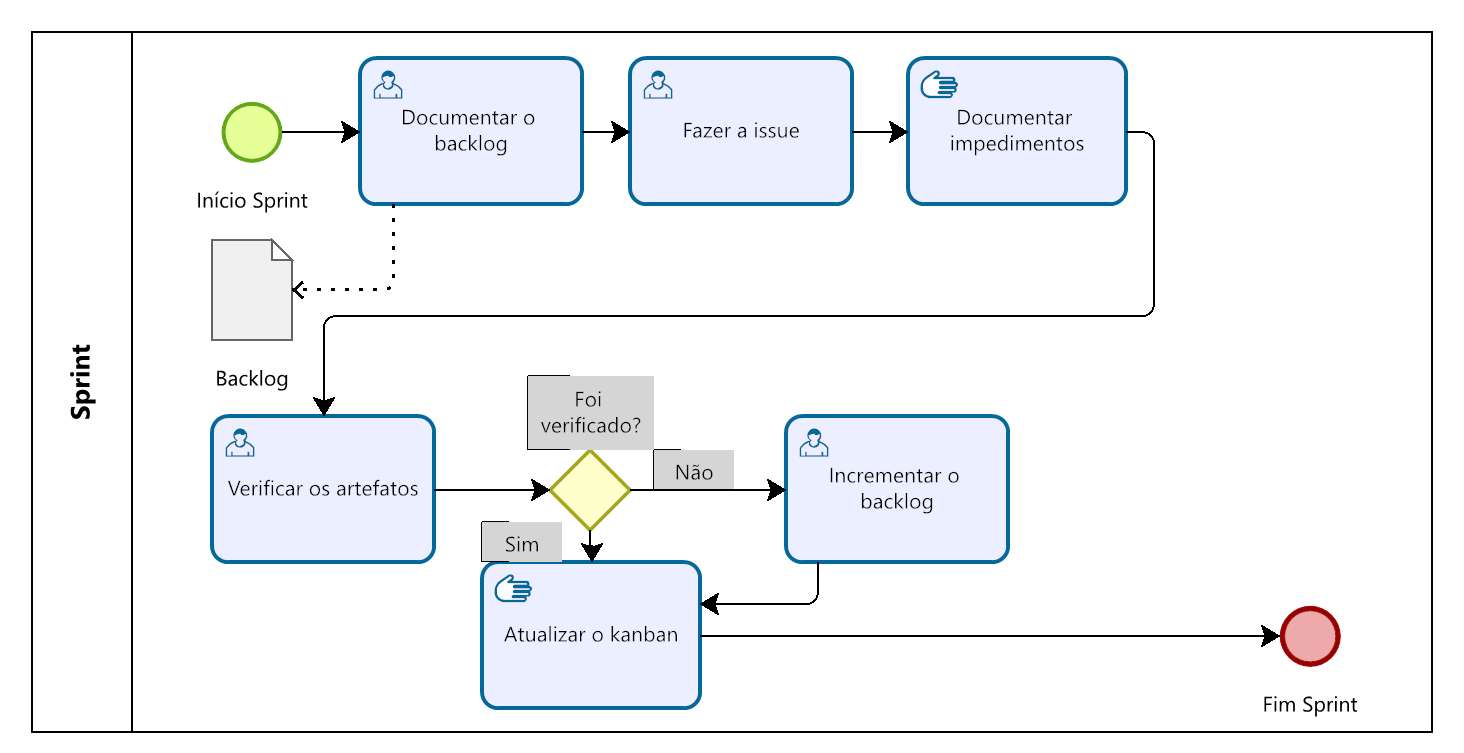
\includegraphics[width=1\linewidth]{Imagens/BPMNSprint.png}
    \par
    Fonte: Autoria própria.
    \par
    \label{fig:bpmn_sprint}
\end{figure}

\subsection{Kanban}

O Kanban é uma metodologia ágil que se concentra na gestão visual do fluxo de trabalho e na limitação do trabalho em progresso. Originado na indústria automobilística japonesa, o Kanban foi adaptado para o desenvolvimento de software, onde o trabalho só é iniciado quando há capacidade disponível na próxima etapa do processo. A ideia central do Kanban é o seu quadro, que divide o trabalho em colunas representando os estágios do processo. Ao visualizar o fluxo, a equipe pode identificar gargalos, reduzir o desperdício de tempo e focar na entrega contínua e rápida de funcionalidades.

Ao limitar o trabalho em progresso, o Kanban impede que a equipe inicie múltiplas tarefas simultaneamente, o que levaria à perda de foco e a longos tempos de ciclo. Essa ideia é crucial para um projeto acadêmico com prazos definidos. Em um estudo sobre o impacto do Kanban na Aprendizagem Baseada em Problemas (ABP), \citeonline{trinidad_2025} concluíram que a aplicação do método Kanban em estudantes universitários demonstrou efeitos positivos, destacando o potencial da ferramenta para organizar e visualizar o desenvolvimento de tarefas complexas em um contexto acadêmico.

Para o desenvolvimento deste trabalho, o Kanban será empregado como um sistema visual de acompanhamento, complementando o framework Scrum e atuando como o principal mecanismo de gestão do fluxo de trabalho. Dessa forma, o quadro Kanban será usado para rastrear o progresso das tarefas de desenvolvimento do aplicativo. A utilização do Kanban permitirá ao desenvolvedor e ao orientador inspecionar o andamento do projeto de forma transparente, facilitando a identificação de quaisquer bloqueios ou atrasos e garantindo que a capacidade de trabalho esteja sempre focada na próxima funcionalidade de maior valor. A seguir está representado o fluxo de atividades da atualização do quadro Kanban do projeto.

\begin{figure}[H]
    \centering
    \caption{BPMN Kanban}
    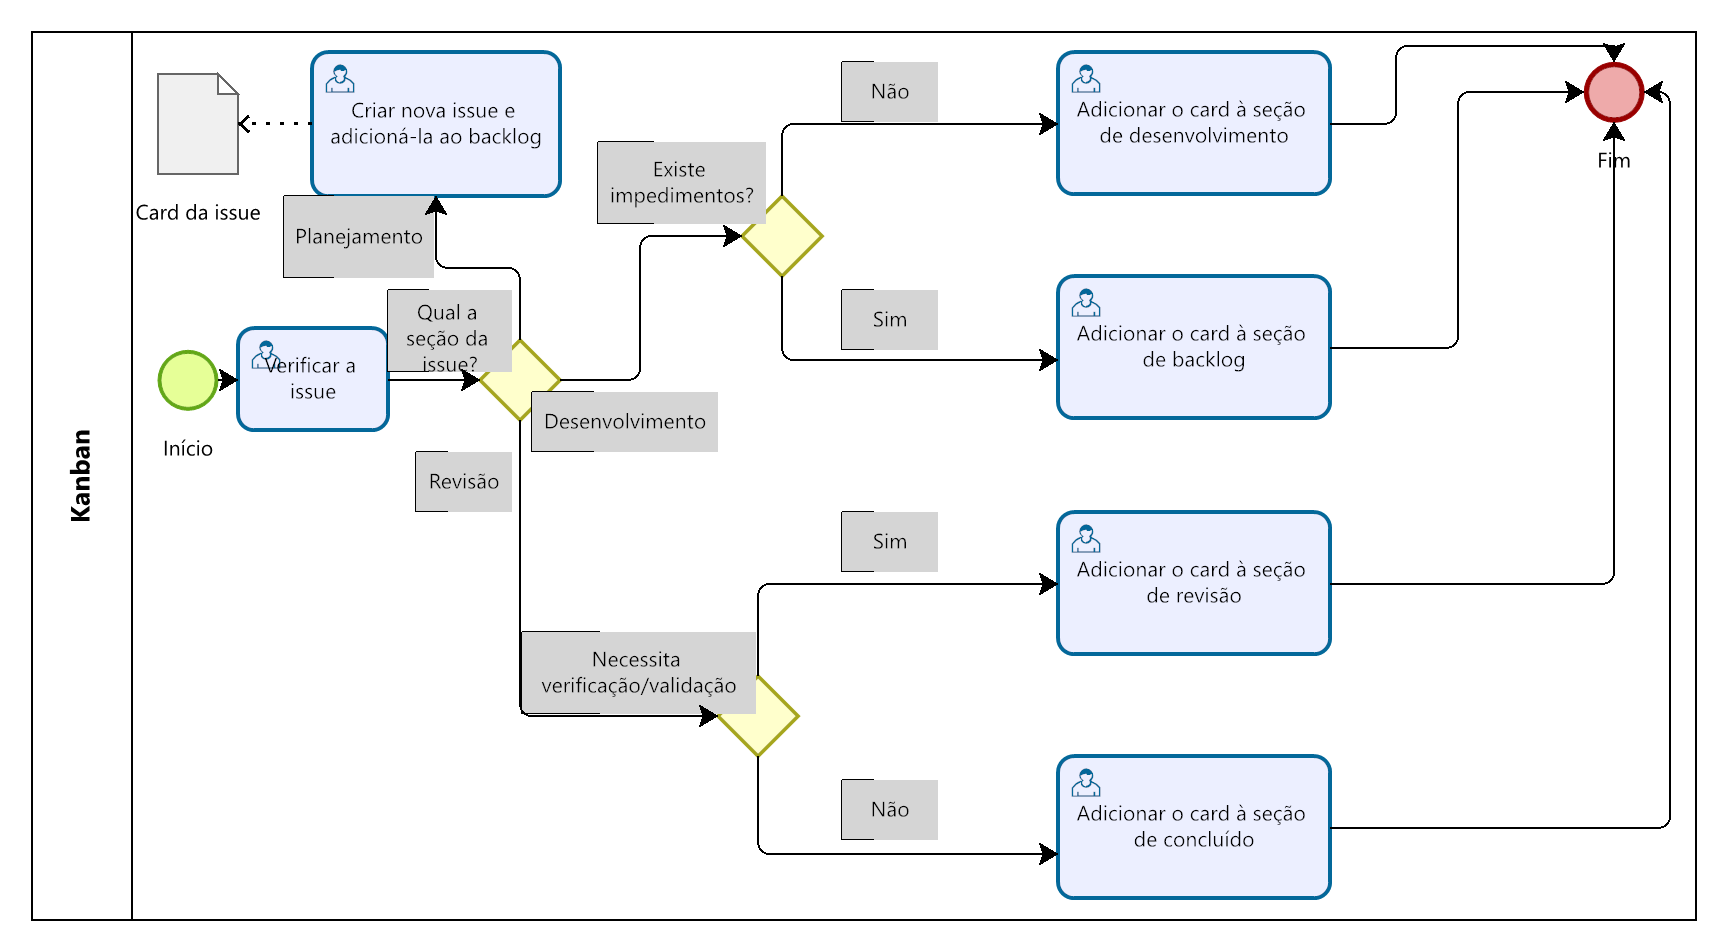
\includegraphics[width=1\linewidth]{Imagens/BPMNKanban.png}
    \par
    Fonte: Autoria própria.
    \par
    \label{fig:bpmn_kanban}
\end{figure}

\subsection{Lean Inception}

O Lean Inception é uma abordagem estruturada, idealizada por Paulo Caroli, que se destina a alinhar o desenvolvedor, os stakeholders e o cliente em torno da visão de um Produto Mínimo Viável (MVP) em um período de tempo. Essa metodologia combina os princípios do Design Thinking, Lean Startup e Metodologias Ágeis. O principal objetivo é garantir que o esforço de desenvolvimento de software comece com uma compreensão clara do problema a ser resolvido e do valor que a solução deve entregar. Em projetos ágeis, onde os requisitos podem evoluir, o Lean Inception atua como uma fase crucial de definição para evitar o desperdício de recursos na construção de funcionalidades desnecessárias.

Dessa forma, as metodologias ágeis às vezes não incluem os usuários finais na participação direta nas etapas iniciais de definição do projeto. Em vez disso, a visão é definida por clientes relacionados apenas ao negócio, o que pode levar a um produto que não atenda às necessidades reais do usuário final. É neste ponto que o Lean Inception se destaca, fornecendo uma série de atividades estruturadas que buscam integrar a perspectiva do usuário desde o início. Conforme apontado por \citeonline{ferreira_2025}, o Lean Inception representa uma metodologia que combina o Design Thinking e o Lean Startup para apoiar a definição do problema focado nas necessidades do usuário e a produção de software eficaz.

Portanto, a adoção do framework Lean Inception é essencial para a fase de planejamento, garantindo que a proposta de valor do aplicativo seja clara, validada e centrada nas necessidades do usuário final. O Lean Inception serve como um guia para transformar os requisitos em artefatos para o desenvolvimento. Ao passar por todas as etapas, o projeto garantirá que o MVP a ser desenvolvido na etapa do TCC2 seja o menor conjunto de funcionalidades capaz de entregar o maior valor possível, reduzindo o risco de construir um produto que não satisfaça as demandas reais do projeto. A estrutura do Lean Inception é a garantia de que o projeto terá uma definição certa do problema e um alto grau de envolvimento do usuário, conforme investigado por \citeonline{ferreira_2025}.

\subsubsection{Kick-off}

O Kick-off é a etapa inicial e fundamental do Lean Inception, atuando como o ponto de partida para alinhar todos os participantes em relação ao propósito e às regras. De acordo com \citeonline{caroli_2017}, o principal objetivo deste momento é garantir que a equipe e os stakeholders compartilhem uma compreensão única sobre o que será feito e sobre o porquê de o projeto existir. Essa seção introdutória é onde são apresentados os participantes, o contexto do projeto, e a agenda das atividades do framework. A clareza alcançada nessa etapa é vital para eliminar ambiguidades e evitar realinhamentos nas próximas fases do desenvolvimento.

Portanto, o Kick-off será conduzido com o próprio autor e o orientador acadêmico, sendo essencial para validar o entendimento do problema e a proposta de valor do aplicativo para os usuários finais. Dessa forma, garantindo que a Visão de Produto seja construída sobre uma base de conhecimento compartilhado e alinhamento de expectativas. Ao finalizar o Kick-off, o projeto estabelece o tom ágil e colaborativo necessário para a construção do MVP, minimizando o risco de que o produto final não reflita os objetivos acadêmicos e as necessidades práticas do usuário, conforme orienta a metodologia \cite{caroli_2017}.

\subsubsection{Visão de Produto}

A Visão de Produto é o primeiro artefato de alto nível que surge do Lean Inception e serve como a idéia estratégica do projeto, englobando o propósito do aplicativo e o impacto que se espera causar no público-alvo. Segundo \citeonline{caroli_2017}, uma visão de produto eficaz deve ser concisa, inspiradora e orientada ao valor, atuando como um guia para a tomada de decisões futuras sobre o que incluir ou excluir do escopo do MVP. Ela responde à pergunta fundamental: "Qual é o produto que vai ser construído e por que ele importa?".

Para estruturar essa visão, o Lean Inception utiliza o formato de template "Visão de Produto" de Geoffrey Moore, que preenche as seguintes perguntas: público-alvo, problema, nome, categoria do produto, principal benefício, concorrentes e diferencial primário. A clareza ao preencher essas perguntas é essencial, pois ela garante que o time de desenvolvimento compreenda o valor de negócio antes de se aprofundar na lista de funcionalidades. A seguir estão documentadas as respostas da visão de produto.

\begin{itemize}
    \item \textbf{Público-alvo:} Estudantes de concursos e estudantes acadêmicos.
    \item \textbf{Problema:} Inexistência de aplicativos gratuitos que integram Timer Pomodoro, Flashcards, Gamificação e Check-ins de humor.
    \item \textbf{Nome:} Focus.
    \item \textbf{Categoria:} Aplicativo mobile.
    \item \textbf{Benefício:} Aprimorar a rotina de estudos do usuário.
    \item \textbf{Concorrentes:} Aprovado e StudyTok.
    \item \textbf{Diferencial:} Integra as diferentes idéias em um único aplicativo gratuito.
\end{itemize}

\subsubsection{É - Não é - Faz - Não faz}

A matriz "É – Não É – Faz – Não Faz" é uma que delimita o escopo do MVP. Esta matriz força a equipe e os stakeholders a criarem clareza e consenso sobre o que o produto será e o que ele fará em sua primeira versão. Segundo \citeonline{caroli_2017}, o uso desta matriz é um exercício de priorização e alinhamento, pois, ao declarar o que o produto não é e o que ele não faz, a equipe está definindo limites cruciais que protegem o projeto contra o desvio de escopo.

A matriz é dividida em quatro quadrantes que exploram a identidade e o comportamento do produto. A coluna "É" define a categoria e a natureza do produto, enquanto a coluna "Não É" estabelece fronteiras sobre o que o aplicativo não contempla. De forma similar, a coluna "Faz" lista as ações principais do produto, já a coluna "Não Faz" lista funcionalidades que poderiam ser esperadas, mas não estão no escopo. A seguir está listada essa matriz para o presente trabalho.

\begin{itemize}
    \item \textbf{É:} Aplicativo mobile, gratuito e open source.
    \item \textbf{Não é:} Um banco de questões para estudo de concursos.
    \item \textbf{Faz:} Integra o Timer Pomodoro, Flashcards, Gamificação e Check-ins de humor para auxiliar na rotina de estudos dos usuários.
    \item \textbf{Não faz:} Não corrige questões, não possui uma base de dados de questões ou conteúdos, não cria atividades, não gera conteúdo e não utiliza inteligência artificial.
\end{itemize}

\subsubsection{Objetivos do Negócio}

Para este trabalho foram acordados os seguintes objetivos de negócio: Eficácia da integração das metodologias, Minimizar a taxa de abandono, Fornecer uma interface intuitiva, Fornecer check-ins de saúde, Seção de progresso e Notificações.

\textbf{Eficácia da integração das metodologias}

Este objetivo será atingido ao entrelaçar o uso da Repetição Espaçada com os ciclos de foco do Timer Pomodoro, garantindo que o estudante revise o material certo no momento ideal.

\textbf{Minimizar a taxa de abandono}

Este objetivo será alcançado através dos elementos de gamificação. Ao utilizar barras de progresso, pontos e badges de conquista, o aplicativo busca transformar o esforço em uma experiência progressiva.

\textbf{Fornecer uma interface intuitiva}

A interface deve ser minimalista, tornando as complexidades do SRS e do Pomodoro transparentes ao usuário. O foco deve estar em simplificar a navegação e a interação, permitindo que o usuário dedique suas energias aos estudos, e não à compreensão de como usar o aplicativo.

\textbf{Fornecer check-ins de saúde}

A funcionalidade permite que o aplicativo monitore o estado psicológico do usuário antes e após as sessões de estudo. Essa informação é vital para o processo de autorregulação.

\textbf{Seção de progresso}

Essa seção deve mostrar o progresso numa visão macro e o avanço dentro de cada disciplina ou tópico.

\subsubsection{Personas}

A atividade de definição de Personas dentro do Lean Inception é um exercício focado no usuário final. Uma Persona é um usuário fictício, mas detalhado e realista, que representa um segmento de usuários. Segundo \citeonline{caroli_2017}, o desenvolvimento de Personas transforma as necessidades abstratas do estudante em características, metas e dores concretas. Ao criar essas representações, a equipe de desenvolvimento consegue tomar decisões de design e funcionalidade baseadas em quem realmente usará o produto e quais são seus desafios específicos, garantindo que o aplicativo seja centrado no usuário. A seguir estão representadas as três personas deste trabalho.

\textbf{Primeira Persona}

\begin{itemize}
    \item Perfil:
    \begin{itemize}
        \item Nome: Icarus.
        \item Idade: 20 anos.
        \item Profissão: Estudante universitário.
    \end{itemize}
    \item Objetivos:
    \begin{itemize}
        \item Minimizar a taxa de abandono.
    \end{itemize}
    \item Frustrações:
    \begin{itemize}
        \item Não sabe por onde começar;
        \item Sofre com a procrastinação e o burnout;
        \item Iniciante na vida acadêmica.
    \end{itemize}
    \item Necessidades:
    \begin{itemize}
        \item Alta necessidade de estrutura e motivação.
    \end{itemize}
\end{itemize}

\textbf{Segunda Persona}

\begin{itemize}
    \item Perfil:
    \begin{itemize}
        \item Nome: Hazel.
        \item Idade: 27 anos.
        \item Profissão: Jornalista.
    \end{itemize}
    \item Objetivos:
    \begin{itemize}
        \item Aprender métodos para tornar suas seções de estudos mais eficazes;
    \end{itemize}
    \item Frustrações:
    \begin{itemize}
        \item Tempo de estudo muito limitado;
        \item Falta de tempo para gerenciar o cronograma;
        \item Dificuldade em reter conteúdo após longas pausas;
        \item Muito ocupada;
    \end{itemize}
    \item Necessidades:
    \begin{itemize}
        \item Eficácia da Integração das Metodologias.
    \end{itemize}
\end{itemize}

\textbf{Terceira Persona}

\begin{itemize}
    \item Perfil:
    \begin{itemize}
        \item Nome: Arabella.
        \item Idade: 25 anos.
        \item Profissão: Estudante universitária.
    \end{itemize}
    \item Objetivos:
    \begin{itemize}
        \item Poder medir sua ansiedade e estresse durante os estudos.
    \end{itemize}
    \item Frustrações:
    \begin{itemize}
        \item Alto volume de conteúdo para revisar e consolidar;
        \item Dificuldade em otimizar as revisões;
        \item Estresse e fadiga mental pelo ritmo.
    \end{itemize}
    \item Necessidades:
    \begin{itemize}
        \item Receber e analisar seus Check-ins de Saúde e usar a Interface Intuitiva.
    \end{itemize}
\end{itemize}

\subsubsection{Jornadas de Usuário}

A atividade de mapeamento das Jornadas de Usuário no Lean Inception consiste em visualizar a sequência de passos, interações e emoções que cada Persona experimenta ao tentar atingir seus objetivos principais utilizando o produto. A seguir estão representadas as três jornadas.

\begin{table}[H]
\centering
\caption{Jornada de Icarus}
\label{tab:jornada_icarus}
\begin{tabular}{|p{2.5cm}|p{2.5cm}|p{2.8cm}|p{3cm}|p{3.5cm}|}
\hline
\textbf{Etapa da Jornada} & \textbf{Ação da Persona (Icarus)} & \textbf{Sentimento} & \textbf{Ponto de Dor / Desafio} & \textbf{Ação do Aplicativo (Funcionalidade)} \\ \hline
1. Início & Precisa começar a estudar, mas não sabe por onde. & Ansiedade / Tédio & Sentimento de sobrecarga e falta de direção. & \textbf{Interface amigável:} Convida o usuário a começar uma seção de estudos. \\ \hline
2. Foco & Inicia a primeira sessão de estudos. & Expectativa & Tendência a se distrair após 10 minutos. & \textbf{Timer Pomodoro:} Inicia ciclo de 25/5 com alerta visual e sonoro. \\ \hline
3. Busca por Motivação & Completa a primeira rodada de estudos. & Satisfação inicial & Necessidade de reforço positivo para continuar o ciclo. & \textbf{Gamificação / Seção de Progresso:} Exibe barra de progresso preenchida e contabiliza pontos/tempo de foco. \\ \hline
4. Manutenção do Ritmo & Vê o progresso diário se acumulando. & Engajamento & Risco de esquecer a revisão dos conteúdos estudados. & \textbf{Notificações:} Alerta para o próximo Pomodoro e agenda automaticamente a revisão no SRS. \\ \hline
\end{tabular}
\par
\vspace{0.5em}
\small Fonte: Autoria própria.
\end{table}

\begin{table}[H]
\centering
\caption{Jornada de Hazel}
\label{tab:jornada_hazel}
\begin{tabular}{|p{2.5cm}|p{2.5cm}|p{2.8cm}|p{3cm}|p{3.5cm}|}
\hline
\textbf{Etapa da Jornada} & \textbf{Ação da Persona (Hazel)} & \textbf{Sentimento} & \textbf{Ponto de Dor / Desafio} & \textbf{Ação do Aplicativo (Funcionalidade)} \\ \hline
1. Planejamento & Tem apenas 2 horas disponíveis para estudar à noite. & Pressa / Stress & Perda de tempo tentando decidir o que revisar para maximizar o retorno. & \textbf{Integração SRS/Pomodoro:} O aplicativo sugere automaticamente o bloco de conteúdo mais urgente para revisão. \\ \hline
2. Execução & Inicia a revisão do tópico sugerido. & Concentração & Dificuldade em manter a disciplina de revisão devido ao cansaço. & \textbf{Timer Pomodoro Adaptado:} Executa um ciclo de foco intenso com flashcards (25 min) seguido de um descanso rápido. \\ \hline
3. Consolidação & Completa as sessões e encerra o dia. & Alívio & Preocupação se o esforço de hoje será retido daqui a uma semana. & \textbf{Algoritmo SRS:} Atualiza o intervalo de repetição do conteúdo revisado para um período mais longo (ex: 7 dias). \\ \hline
4. Check-in de Revisão & Recebe notificação de revisão programada. & Confiança & Risco de esquecer o agendamento no meio da rotina. & \textbf{Notificações:} Alerta no momento exato da revisão, eliminando a gestão manual do cronograma. \\ \hline
\end{tabular}
\par
\vspace{0.5em}
\small Fonte: Autoria própria.
\end{table}

\begin{table}[H]
\centering
\caption{Jornada de Arabella}
\label{tab:jornada_arabella}
\begin{tabular}{|p{2.5cm}|p{2.5cm}|p{2.8cm}|p{3cm}|p{3.5cm}|}
\hline
\textbf{Etapa da Jornada} & \textbf{Ação da Persona (Arabella)} & \textbf{Sentimento} & \textbf{Ponto de Dor / Desafio} & \textbf{Ação do Aplicativo (Funcionalidade)} \\ \hline
1. Avaliação do Humor & Prepara-se para uma longa sessão de revisão. & Fadiga / Ansiedade & Não sabe se está em condições emocionais de absorver conteúdo complexo. & \textbf{Check-in de Saúde:} Solicita ao usuário que avalie seu humor e nível de estresse (escala de 1 a 5). \\ \hline
2. Estudo Adaptado & Recebe a sugestão de plano para o dia. & Aceitação & Iniciar um tópico muito difícil pode causar mais estresse. & \textbf{Sugestão de Bem-Estar:} Oferece um plano de revisão mais leve ou sugere uma pausa de 15 minutos baseada no alto índice de estresse reportado. \\ \hline
3. Revisão & Executa a revisão via flashcards. & Foco & Perder tempo procurando o próximo conteúdo a revisar. & \textbf{Interface Intuitiva / SRS:} Apresenta o flashcard mais crítico na tela de forma clara, com botões visuais para a autoavaliação (fácil/difícil). \\ \hline
4. Reflexão Pós-Sessão & Termina o bloco de estudo. & Alívio & Necessidade de ver o impacto das emoções no desempenho. & \textbf{Relatório de Check-in e Progresso:} Exibe a correlação entre o humor inicial e a quantidade de flashcards revisados, fechando o ciclo da Aprendizagem Autorregulada. \\ \hline
\end{tabular}
\par
\vspace{0.5em}
\small Fonte: Autoria própria.
\end{table}

\subsubsection{Brainstorming de Funcionalidades}

A partir das personas, objetivos e necessidades pode-se começar a etapa de brainstorming de funcionalidades. O objetivo desta atividade é gerar um grande número de ideias em um tempo pequeno incentivando a criatividade. O processo começa com a releitura das Jornadas de Usuário, e para cada passo crítico da jornada, os participantes sugerem funcionalidades que ajudariam a Persona a ter uma melhor experiência. A seguir está representado o quadro com todas as ideias iniciais.

\begin{figure}[H]
    \centering
    \caption{Quadro do Brainstorming de Funcionalidades}
    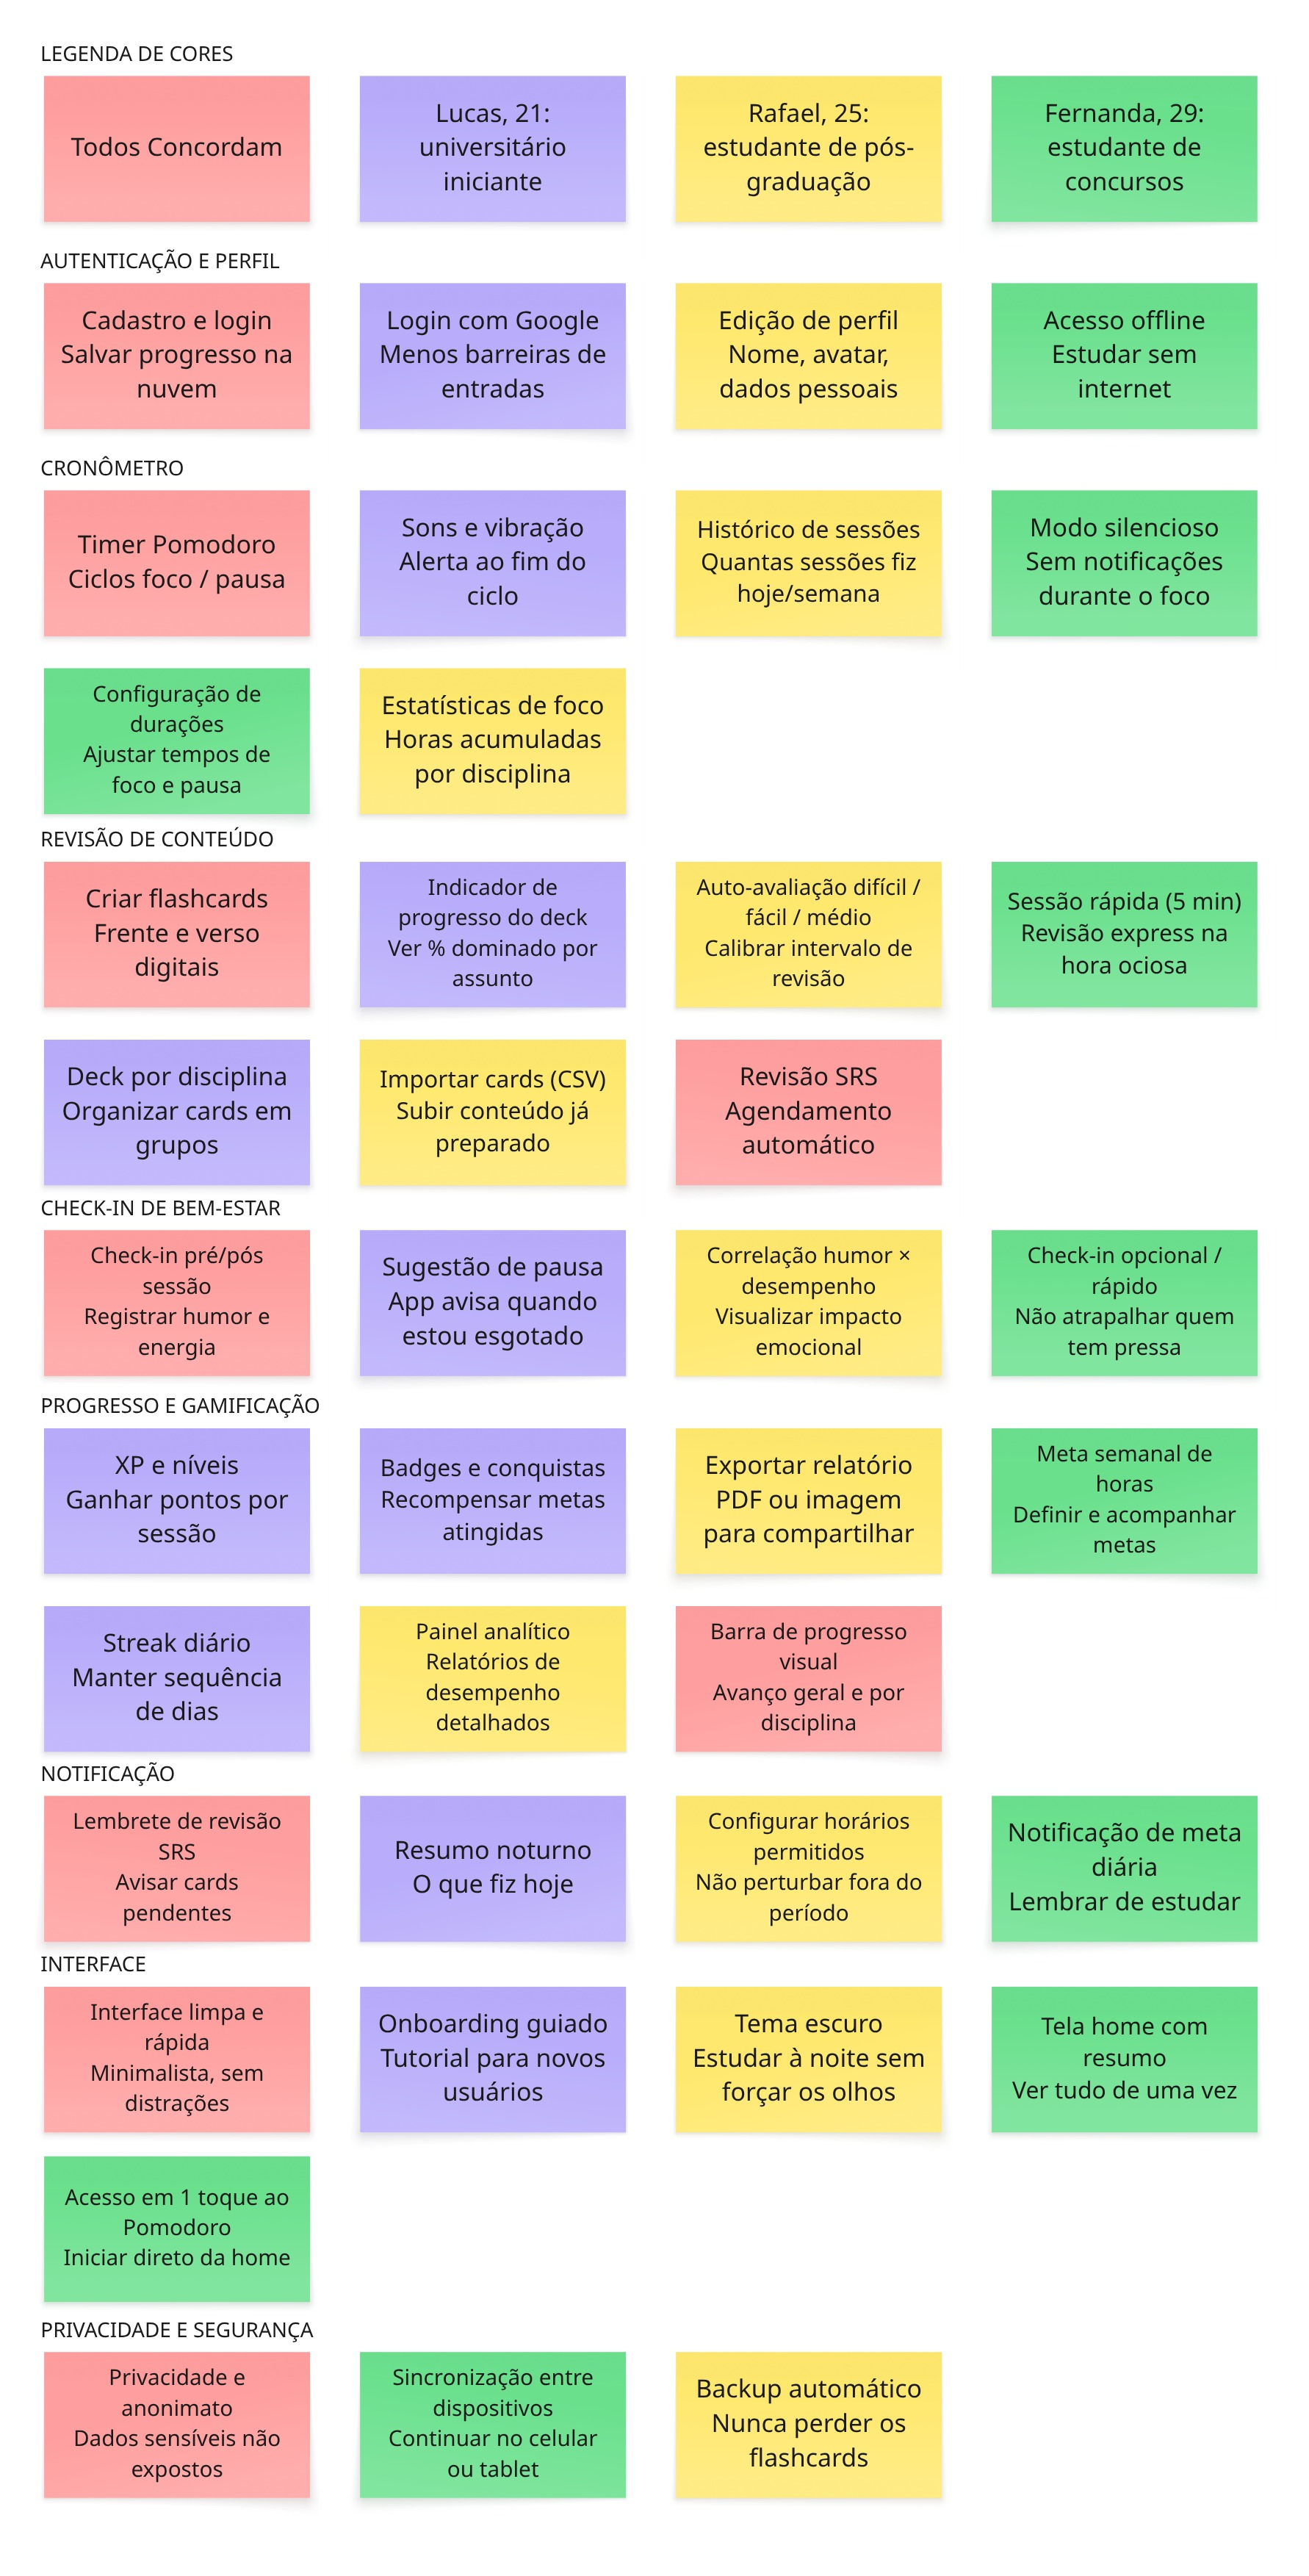
\includegraphics[width=1\linewidth, height=0.9\textheight, keepaspectratio]{Imagens/BrainstormingFuncionalidades.jpg}
    \par
    Fonte: Autoria Própria.
    \par
    \label{fig:brainstorming}
\end{figure}

\FloatBarrier
{\titlespacing*{\subsubsection}{0pt}{0pt}{6pt}
\subsubsection{Revisão Técnica, de Negócio e de Experiência do Usuário}
}

A revisão de negócio atua como o primeiro filtro, questionando o valor de cada funcionalidade sob a ótica dos Objetivos de Negócio definidos anteriormente. A análise é feita inserindo de um a três símbolos de dólar em cada ideia, conforme seu nível técnico.

Em seguida, a revisão técnica e a revisão de experiência do usuário (UX) agem como filtros de viabilidade e desejabilidade. A revisão técnica avalia a complexidade e o esforço de implementação de cada funcionalidade, considerando os recursos disponíveis. Para medir, deve-se inserir de um a três símbolos de esforço (letra E) conforme o nível do esforço em cada ideia. Já a revisão de experiência do usuário (UX), essencial para manter o foco no usuário, avalia se a funcionalidade é simples de usar e se ela resolve o problema da Persona de forma eficaz. Da mesma forma, a medição é feita inserindo de um a três símbolos de coração em cada ideia, conforme seus níveis.

Após essa avaliação, devemos reagrupar as idéias em áreas específicas conforme sua agregação ao escopo do projeto, no chamado Gráfico do Semáforo, segundo \citeonline{caroli_2017}. Onde, as idéias agrupadas na zona crítica, três quadrantes do canto inferior esquerdo, serão excluídas do escopo enquanto as demais permanecem. A seguir está representado o Gráfico do Semáforo deste trabalho.

\begin{figure}[H]
    \centering
    \caption{Gráfico do Semáforo}
    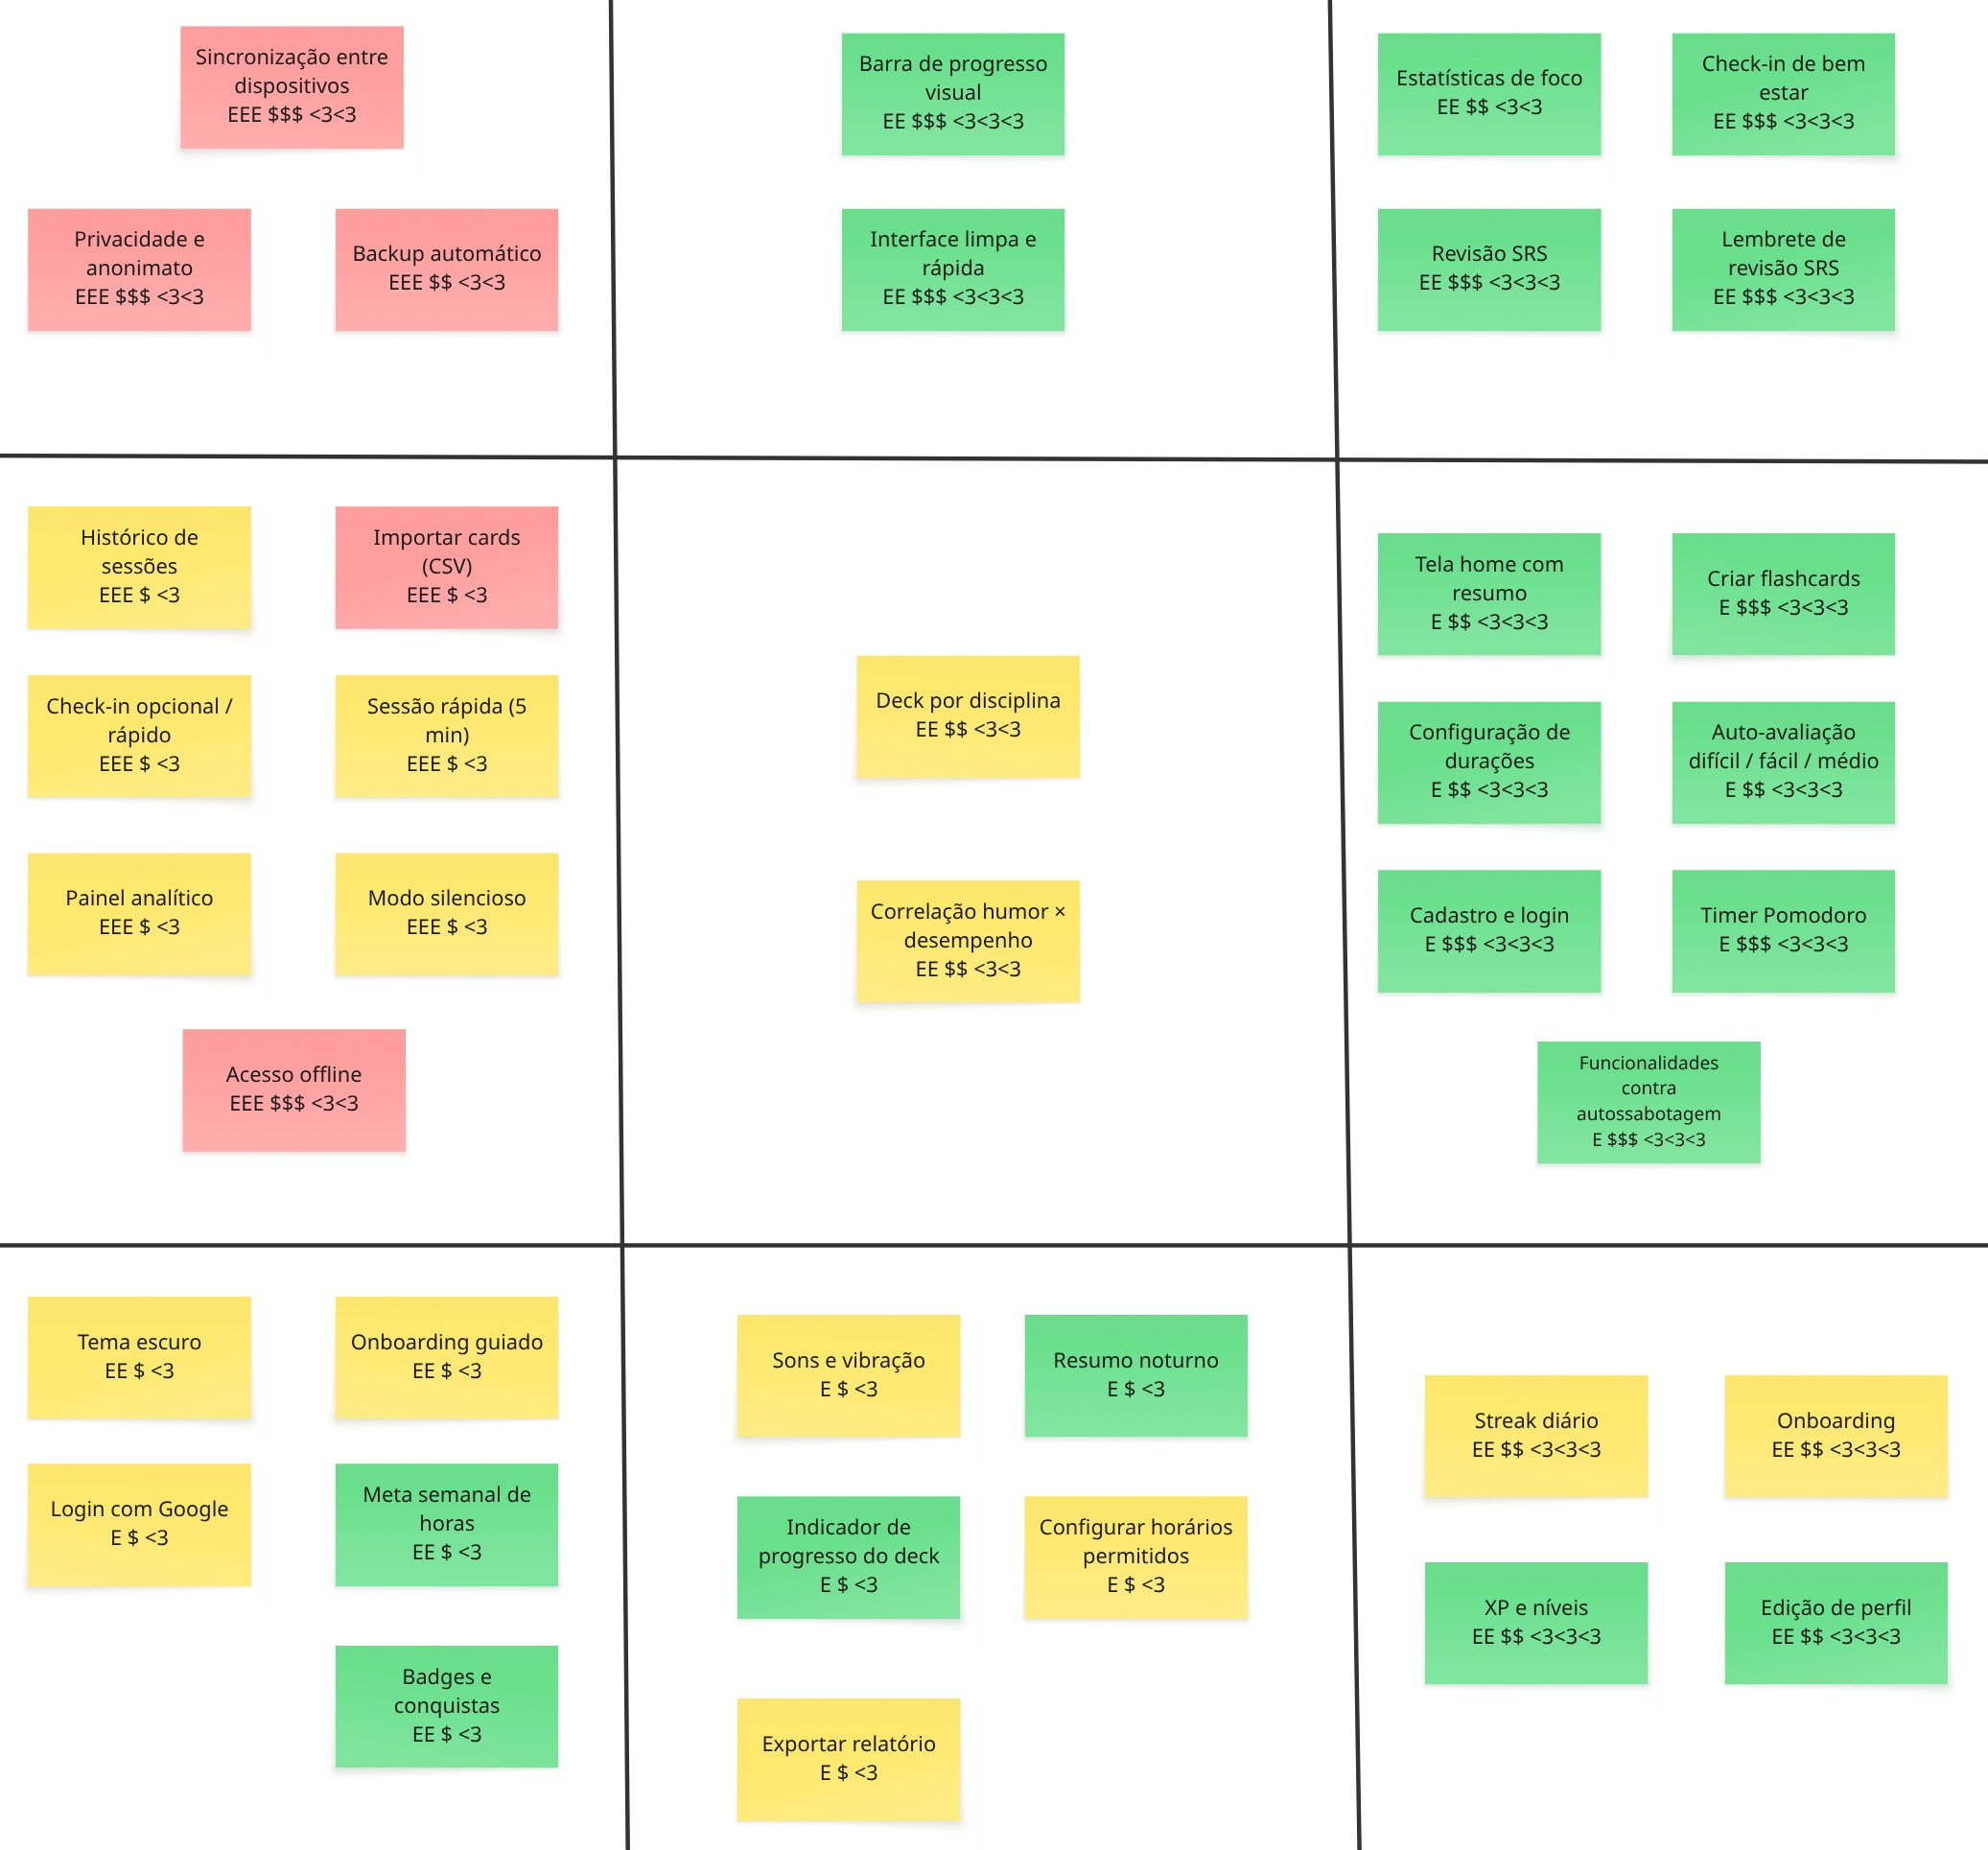
\includegraphics[width=1\linewidth, height=0.9\textheight, keepaspectratio]{Imagens/GraficoSemaforo.jpg}
    \par
    Fonte: Autoria Própria.
    \par
    \label{fig:semaforo}
\end{figure}

\subsubsection{Sequenciador}

O sequenciador é a ferramenta do Lean Inception responsável por dizer a ordem de implementação das funcionalidades, alocando-as em uma linha do tempo composta por ondas. O propósito dessa organização é garantir que o trabalho seja distribuído de maneira incremental e equilibrada, prevenindo a sobrecarga do desenvolvedor e assegurando que o produto evolua de forma sustentável. Conforme \citeonline{caroli_2017}, o sequenciamento não é aleatório, ele deve respeitar regras lógicas que levam em conta o valor entregue ao usuário e sua complexidade técnica para cada item.

Para assegurar esse equilíbrio, cada onda de desenvolvimento deve aderir a alguns critérios de formação. Primeiramente, limita-se a densidade de, no máximo, três funcionalidades por onda. Também não se pode ter uma onda composta exclusivamente por itens de alto esforço, sendo permitido, no máximo, um cartão vermelho por ciclo. Além disso, a soma total do esforço técnico por onda deve ser limitada a 5 pontos, garantindo que o volume de trabalho seja coerente.

Cada onda deve atingir uma soma mínima de 4 pontos tanto para o valor de negócio quanto para a experiência do usuário (UX), assegurando que nenhum ciclo de desenvolvimento irá ser somente técnico ou sem utilidade para o cliente final. Por fim, a metodologia exige atenção à arquitetura do software, determinando que funcionalidades com dependências técnicas diretas sejam alocadas em ondas diferentes.

\begin{figure}[H]
    \centering
    \caption{Sequenciador}
    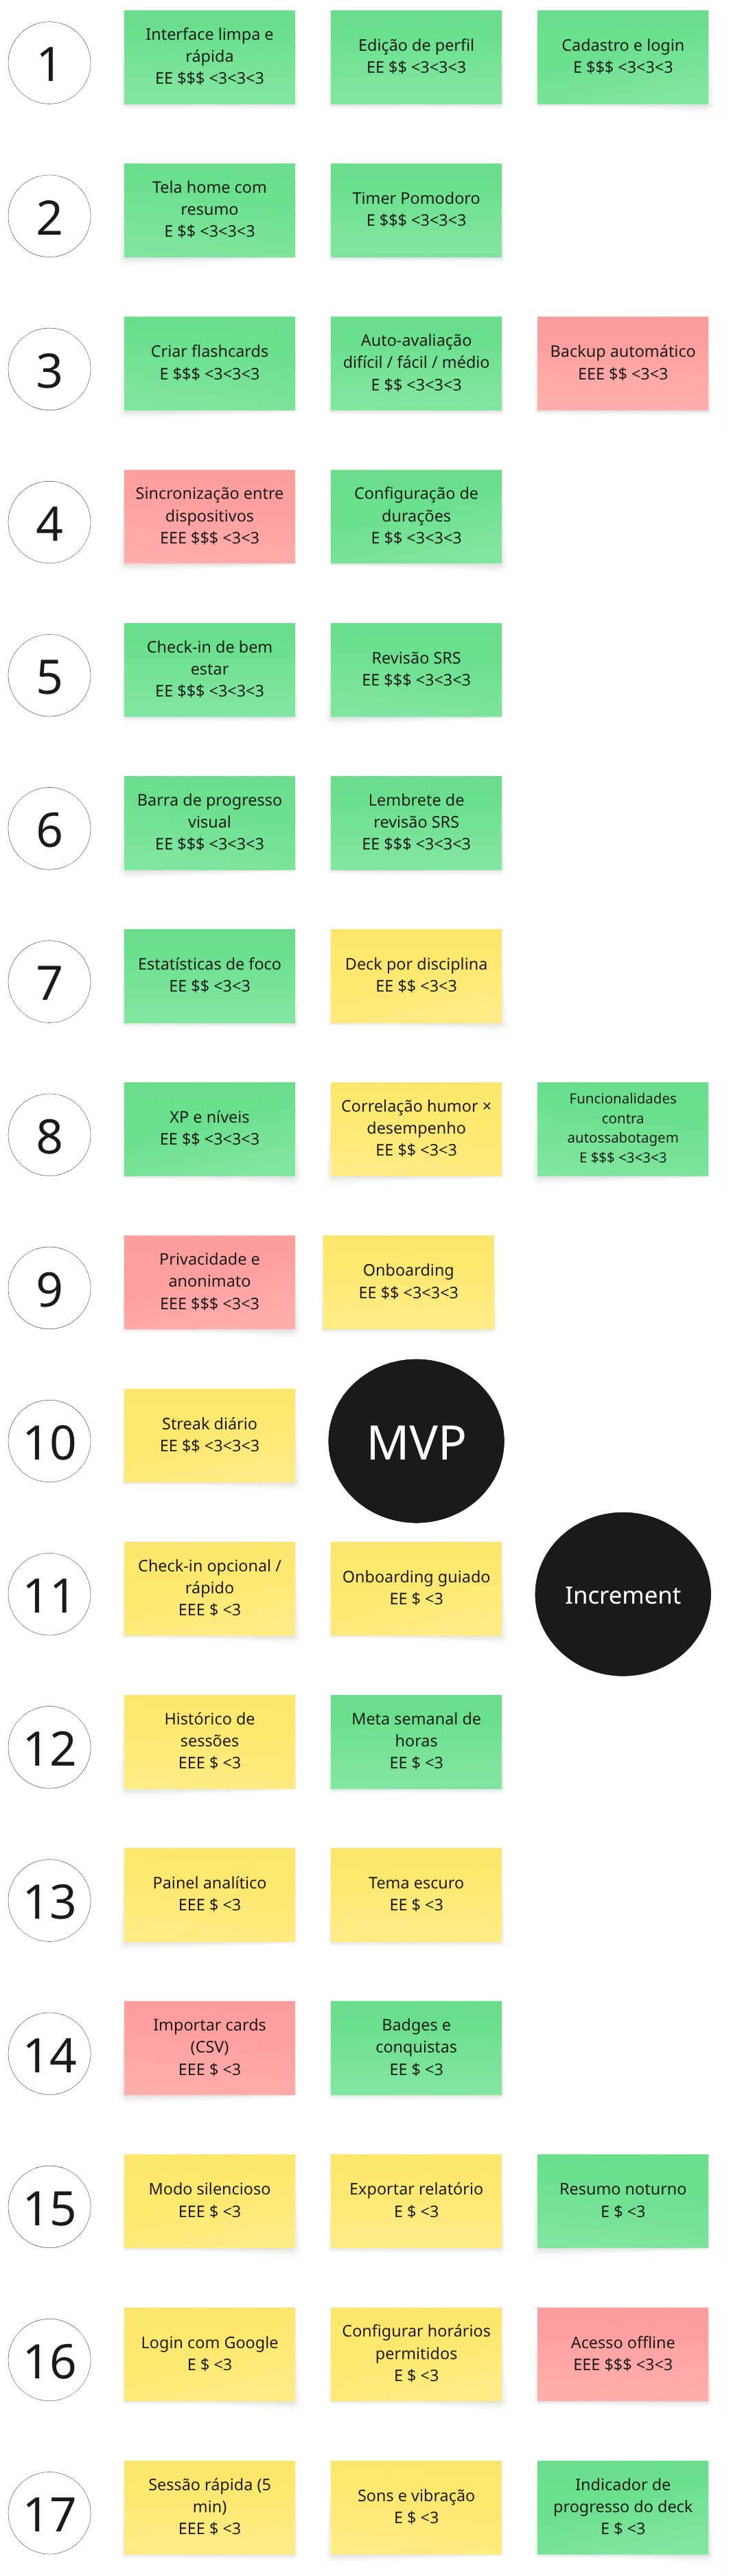
\includegraphics[width=0.8\linewidth, height=0.85\textheight, keepaspectratio]{Imagens/Sequenciador.jpg}
    \par
    Fonte: Autoria própria.
    \par
    \label{fig:sequenciador}
\end{figure}

\subsubsection{Canvas MVP}

Finalmente, a última etapa do Lean Inception é a elaboração do Canvas MVP, um quadro visual que sintetiza as decisões estratégicas do workshop para garantir o alinhamento sobre o que será construído e como o sucesso será medido. De acordo com \citeonline{caroli_2017}, este artefato condensa a essência do produto mínimo viável em sete componentes fundamentais: a definição clara da proposta do MVP, a identificação das personas atendidas e suas respectivas jornadas, a listagem das funcionalidades prioritárias, os resultados almejados e as métricas para a validação das hipóteses de negócio, finalizando com a estimativa de custos e o cronograma previsto. A seguir está representado o canvas MVP deste trabalho.

\begin{figure}[H]
    \centering
    \caption{Canvas MVP}
    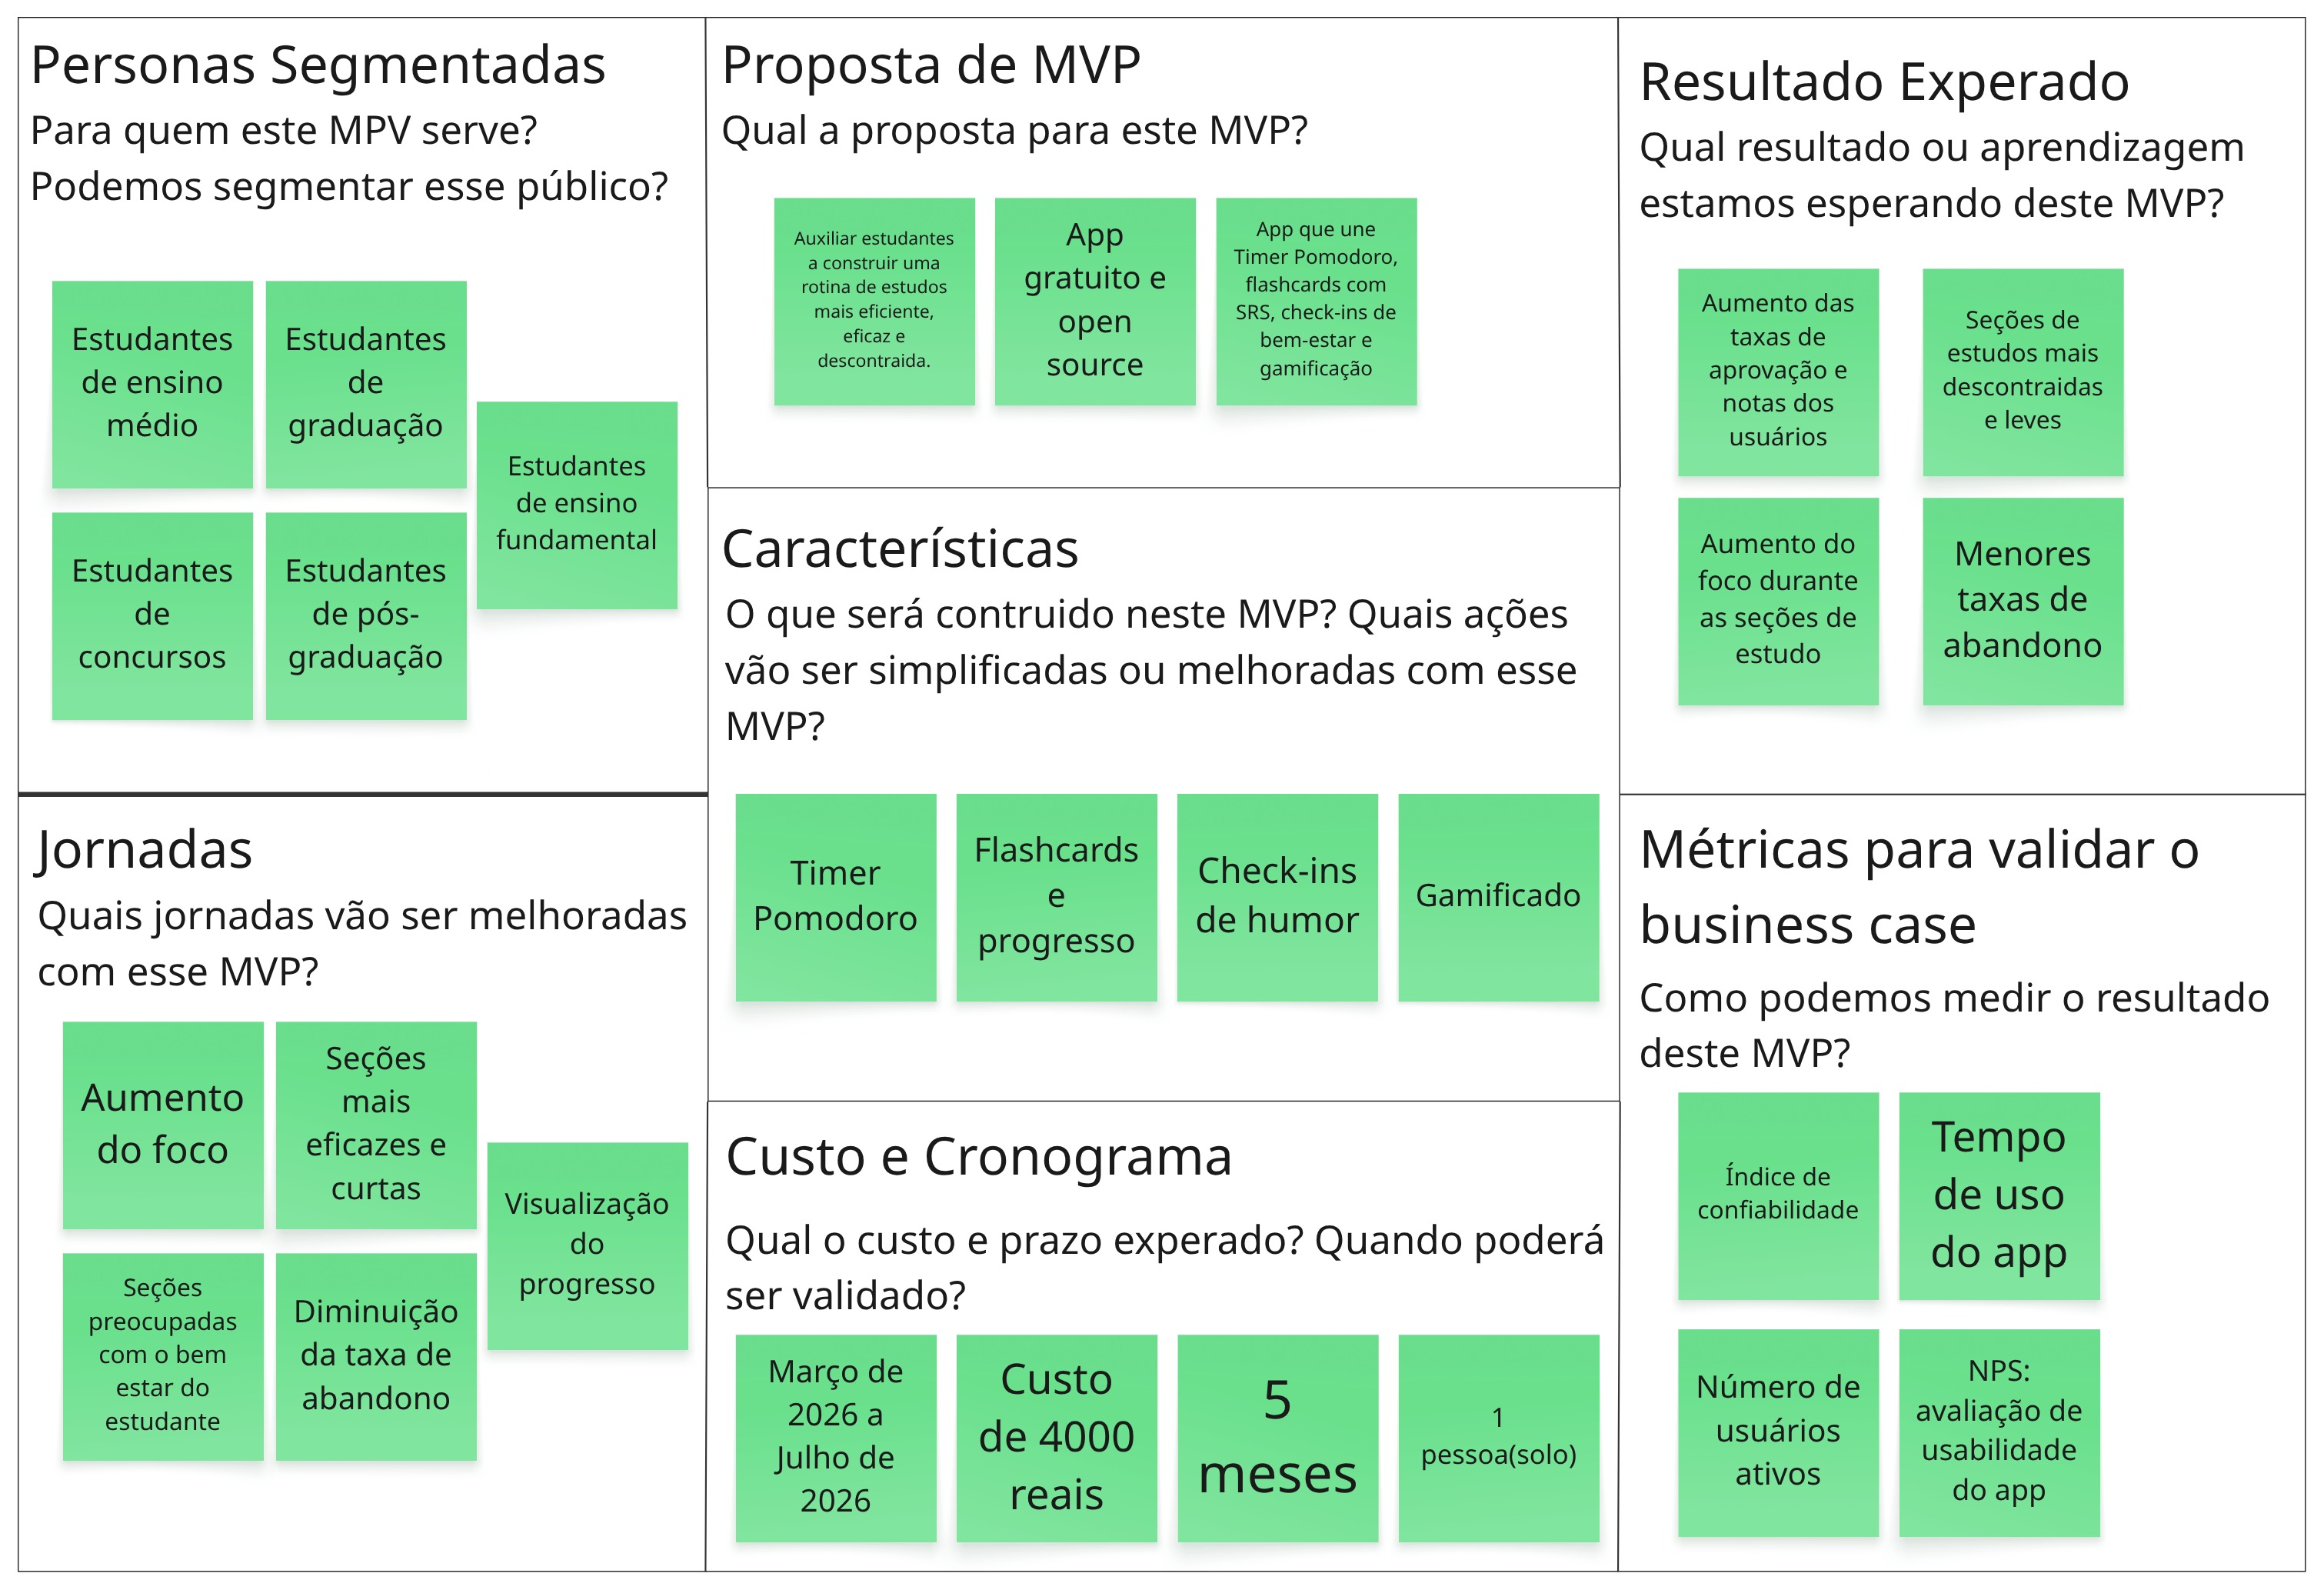
\includegraphics[width=1\linewidth]{Imagens/CanvasMVP.jpg}
    \par
    Fonte: Autoria própria.
    \par
    \label{fig:canvas_mvp}
\end{figure}

\section{Requisitos}

Os requisitos são especificações do sistema que visam suprir as necessidades dos usuários, sendo a sua elicitação uma etapa crucial para o desenvolvimento de software. De acordo com \citeonline{khalid_2025}, requisitos mal gerenciados são uma das principais causas de falha em projetos de software e aumento de custos, o que torna a engenharia de requisitos uma fase fundamental para garantir a qualidade e a satisfação do usuário final.

Sendo assim, para este projeto, foram utilizados artefatos do workshop Lean Inception, como Personas, Brainstorming de Funcionalidades e Jornadas de Usuário para elicitar os requisitos. Além disso, utilizou-se o método MoSCoW para a priorização das funcionalidades levantadas, proporcionando uma visão do que compõe o MVP e garantindo que o desenvolvimento foque no valor do aplicativo.

\subsection{Requisitos Funcionais}

Os requisitos funcionais representam as funcionalidades que o sistema deve oferecer para atender às necessidades dos usuários. Eles descrevem comportamentos, serviços e regras de negócio que o sistema deverá executar para auxiliar o estudante em sua jornada de preparação.

\subsubsection{Histórias de Usuário}

As histórias de usuário têm como principal objetivo descrever as funcionalidades necessárias do ponto de vista do usuário. Para este projeto, elas foram divididas em épicos, que representam grandes conjuntos de funcionalidades, e features, que são funcionalidades específicas derivadas desses épicos.

A fim de proporcionar maior controle sobre o escopo do MVP, utilizou-se o método de priorização MoSCoW, que classifica os requisitos nas seguintes categorias:

\begin{itemize}
    \item \textbf{Must (Deve ter):} requisitos obrigatórios para o funcionamento do MVP;
    \item \textbf{Should (Deveria ter):} requisitos importantes, mas que podem ser postergados;
    \item \textbf{Could (Poderia ter):} requisitos desejáveis, mas não essenciais no momento;
    \item \textbf{Won't (Não terá):} requisitos que não serão implementados nesta versão.
\end{itemize}

A seguir, apresentam-se as funcionalidades desenvolvidas usando histórias de usuário (US) e priorizadas com MoSCoW.

\textbf{Épico 1 --- Gerenciamento de Usuário e Perfil}

\begin{itemize}
    \item \textbf{Feature F01: Registro e Acesso.}
    \begin{itemize}
        \item \textit{US01:} Eu, como usuário, desejo me cadastrar informando nome, e-mail e senha, e realizar login no aplicativo, para que meu progresso de estudo seja salvo na nuvem e acessível de qualquer dispositivo.
        \item \textit{Prioridade:} deve ter.
    \end{itemize}
    \item \textbf{Feature F02: Edição de Perfil.}
    \begin{itemize}
        \item \textit{US02:} Eu, como usuário, desejo editar meu nome no aplicativo, para que minhas informações pessoais estejam sempre atualizadas.
        \item \textit{Prioridade:} deveria ter.
    \end{itemize}
\end{itemize}

\textbf{Épico 2 --- Gestão do Ciclo de Estudo}

\begin{itemize}
    \item \textbf{Feature F03: Timer Pomodoro.}
    \begin{itemize}
        \item \textit{US03:} Eu, como usuário, desejo iniciar um cronômetro de foco e descanso configurável (duração e número de ciclos) para gerenciar meu tempo de estudo com a Técnica Pomodoro.
        \item \textit{Prioridade:} deve ter.
    \end{itemize}
    \item \textbf{Feature F04: Algoritmo de Repetição Espaçada (SRS).}
    \begin{itemize}
        \item \textit{US04:} Eu, como usuário, desejo avaliar a dificuldade de um flashcard revisado (Fácil, Difícil, Errei, etc.) para que o sistema agende automaticamente a próxima revisão com base no meu desempenho.
        \item \textit{Prioridade:} deve ter.
    \end{itemize}
    \item \textbf{Feature F05: Listagem de Revisões Pendentes.}
    \begin{itemize}
        \item \textit{US05:} Eu, como usuário, desejo visualizar na tela inicial (Dashboard) quais flashcards precisam ser revisados hoje conforme o cronograma SRS, para que eu organize minha sessão de estudos.
        \item \textit{Prioridade:} deve ter.
    \end{itemize}
\end{itemize}

\textbf{Épico 3 --- Gerenciamento de Flashcards}

\begin{itemize}
    \item \textbf{Feature F06: Criação, Edição e Exclusão de Flashcards.}
    \begin{itemize}
        \item \textit{US06:} Eu, como usuário, desejo criar flashcards com frente (pergunta) e verso (resposta), bem como editar e excluir cards existentes, para que eu possa montar meu próprio banco de conteúdo de estudo.
        \item \textit{Prioridade:} deve ter.
    \end{itemize}
    \item \textbf{Feature F07: Sessão de Revisão de Flashcards.}
    \begin{itemize}
        \item \textit{US07:} Eu, como usuário, desejo iniciar uma sessão de revisão onde os flashcards são exibidos um a um (frente $\rightarrow$ virar $\rightarrow$ verso $\rightarrow$ avaliar dificuldade).
        \item \textit{Prioridade:} deve ter.
    \end{itemize}
\end{itemize}

\textbf{Épico 4 --- Monitoramento de Bem-Estar e Saúde}

\begin{itemize}
    \item \textbf{Feature F08: Check-in de Saúde.}
    \begin{itemize}
        \item \textit{US08:} Eu, como usuário, desejo registrar diariamente meu nível de humor e estresse por meio de um check-in rápido no Dashboard, para monitorar meu bem-estar emocional ao longo dos estudos.
        \item \textit{Prioridade:} deve ter.
    \end{itemize}
    \item \textbf{Feature F09: Relatórios de Bem-Estar.}
    \begin{itemize}
        \item \textit{US09:} Eu, como usuário, desejo visualizar na tela de Progresso gráficos que mostrem a evolução do meu humor e seu relacionamento com meu desempenho nos flashcards ao longo do tempo.
        \item \textit{Prioridade:} deveria ter.
    \end{itemize}
\end{itemize}

\textbf{Épico 5 --- Gamificação e Engajamento}

\begin{itemize}
    \item \textbf{Feature F10: Sistema de XP, Níveis e Streaks.}
    \begin{itemize}
        \item \textit{US10:} Eu, como usuário, desejo ganhar pontos de experiência (XP) ao completar ciclos Pomodoro e sessões de revisão de flashcards, e visualizar meu nível atual e sequência de dias (streak) na tela de Perfil.
        \item \textit{Prioridade:} deveria ter.
    \end{itemize}
    \item \textbf{Feature F11: Visualização de Progresso.}
    \begin{itemize}
        \item \textit{US11:} Eu, como usuário, desejo visualizar na tela de Progresso gráficos e indicadores sobre meu desempenho.
        \item \textit{Prioridade:} deveria ter.
    \end{itemize}
\end{itemize}

Portanto, a seguir estão representados todos os requisitos funcionais deste trabalho.

\begin{table}[H]
\centering
\caption{Requisitos Funcionais}
\label{tab:requisitosfunc}
\begin{tabularx}{\textwidth}{|c|X|}
\hline
\textbf{ID} & \textbf{Descrição} \\
\hline
FUNC01 & Cadastro e autenticação de usuário. \\
\hline
FUNC02 & Edição de dados cadastrais do perfil. \\
\hline
FUNC03 & Gerenciamento de ciclos de foco e descanso configuráveis. \\
\hline
FUNC04 & Criação, edição e exclusão de flashcards com frente e verso. \\
\hline
FUNC05 & Sessão de revisão de flashcards com flip de carta e avaliação de dificuldade. \\
\hline
FUNC06 & Agendamento automático de revisões baseado no algoritmo SRS e no feedback de dificuldade. \\
\hline
FUNC07 & Listagem de flashcards pendentes de revisão. \\
\hline
FUNC08 & Registro de check-in de humor e nível de estresse. \\
\hline
FUNC09 & Visualização de estatísticas de desempenho. \\
\hline
FUNC10 & Visualização de dados de bem-estar. \\
\hline
FUNC11 & Sistema de gamificação com pontuação por XP, níveis e streak de dias consecutivos. \\
\hline
\multicolumn{2}{r}{\small Fonte: Autoria própria.} \\
\end{tabularx}
\end{table}

\subsection{Requisitos Não Funcionais}

Os requisitos não funcionais são especificações que não se referem diretamente às funcionalidades específicas do sistema, mas sim a como o software deve funcionar. Segundo \citeonline{sommerville_2011}, esses requisitos descrevem restrições e propriedades do sistema, como desempenho, segurança e usabilidade, sendo essenciais para a aceitação do produto. Dessa maneira, \citeonline{gobov_2025} destacam que os atributos de qualidade de software são determinantes para o valor do produto final, e a falta desses requisitos durante a engenharia de software é uma das causas primárias de insatisfação do usuário e de falhas.

\subsubsection{FURPS+}

Para organizar os requisitos não funcionais do projeto, utilizou-se o modelo FURPS+. Este modelo, adotado no Rational Unified Process, categoriza os atributos de qualidade em cinco dimensões principais, além de uma extensão para restrições adicionais:

\begin{itemize}
    \item \textbf{Functionality:} Trata dos requisitos funcionais, já abordados.
    \item \textbf{Usability:} Refere-se à facilidade de uso, design da interface e experiência do usuário (UX). Segundo \citeonline{gobov_2025}, a usabilidade é um atributo externo crítico que impacta diretamente a produtividade do usuário.
    \item \textbf{Reliability:} Trata da confiabilidade, incluindo frequência de falhas, capacidade de recuperação e integridade dos dados.
    \item \textbf{Performance:} Refere-se a eficiência do sistema, como tempo de resposta e consumo de recursos.
    \item \textbf{Supportability:} Refere-se a facilidade de manutenção, testabilidade e portabilidade do software.
    \item \textbf{Plus:} Inclui restrições de implementação, interface, requisitos físicos e observações legais.
\end{itemize}

A partir das métricas de qualidade sugeridas por \citeonline{gobov_2025}, os requisitos não funcionais do aplicativo foram identificados e classificados na Tabela~\ref{tab:requisitosnaofunc}.

\begin{table}[H]
\centering
\caption{Requisitos Não Funcionais}
\label{tab:requisitosnaofunc}
\begin{tabularx}{\textwidth}{|c|X|}
\hline
\textbf{ID} & \textbf{Descrição} \\
\hline
USAB01 & A interface deve seguir uma interface minimalista que garante consistência visual e redução da carga cognitiva. \\
\hline
USAB02 & O aplicativo deve fornecer feedback visual claro ao iniciar, pausar e finalizar ciclos Pomodoro. \\
\hline
USAB03 & O sistema deve seguir padrões de acessibilidade para garantir o uso por diferentes perfis de usuários. \\
\hline
USAB04 & O fluxo completo de resposta a um flashcard deve ser executável com no máximo dois toques na tela. \\
\hline
USAB05 & O check-in de humor deve ser concluído em no máximo três interações a partir do Dashboard. \\
\hline
CONF01 & O sistema deve garantir a persistência dos dados do usuário mesmo após reinicialização do dispositivo. \\
\hline
CONF02 & O aplicativo deve estar em conformidade com a Lei Geral de Proteção de Dados (LGPD), coletando apenas dados necessários. \\
\hline
CONF03 & O sistema deve garantir disponibilidade mínima de 99\% do tempo. \\
\hline
PERF01 & O acionamento e a pausa do cronômetro Pomodoro devem ser instantâneos (tempo de resposta < 500ms). \\
\hline
PERF02 & O cálculo do próximo agendamento pelo algoritmo SRS não deve exceder 1 segundo por flashcard avaliado. \\
\hline
PERF03 & O aplicativo deve sincronizar dados com o servidor em menos de 5 segundos sob conexão estável. \\
\hline
SUPO01 & O aplicativo deve operar no sistema operacional Android. \\
\hline
SUPO02 & O código-fonte deve ser documentado, modular e organizado. \\
\hline
SUPO03 & O sistema deve suportar atualizações do banco de dados sem necessidade de reinstalação do aplicativo. \\
\hline
PLUS01 & O aplicativo deve ocupar, preferencialmente, menos de 100 MB de armazenamento no dispositivo. \\
\hline
\multicolumn{2}{r}{\small Fonte: Autoria própria.} \\
\end{tabularx}
\end{table}
